\chapter{Proposed Application}\label{intro}

    This chapter is an appendix of application screenshot,
    which shows application's interface, functions and the result of the application.
    The application features and usage are decribed in chapter 3.

    \begin{figure}[h!]
        \centering
        \begin{subfigure}{.5\textwidth}
        \centering
        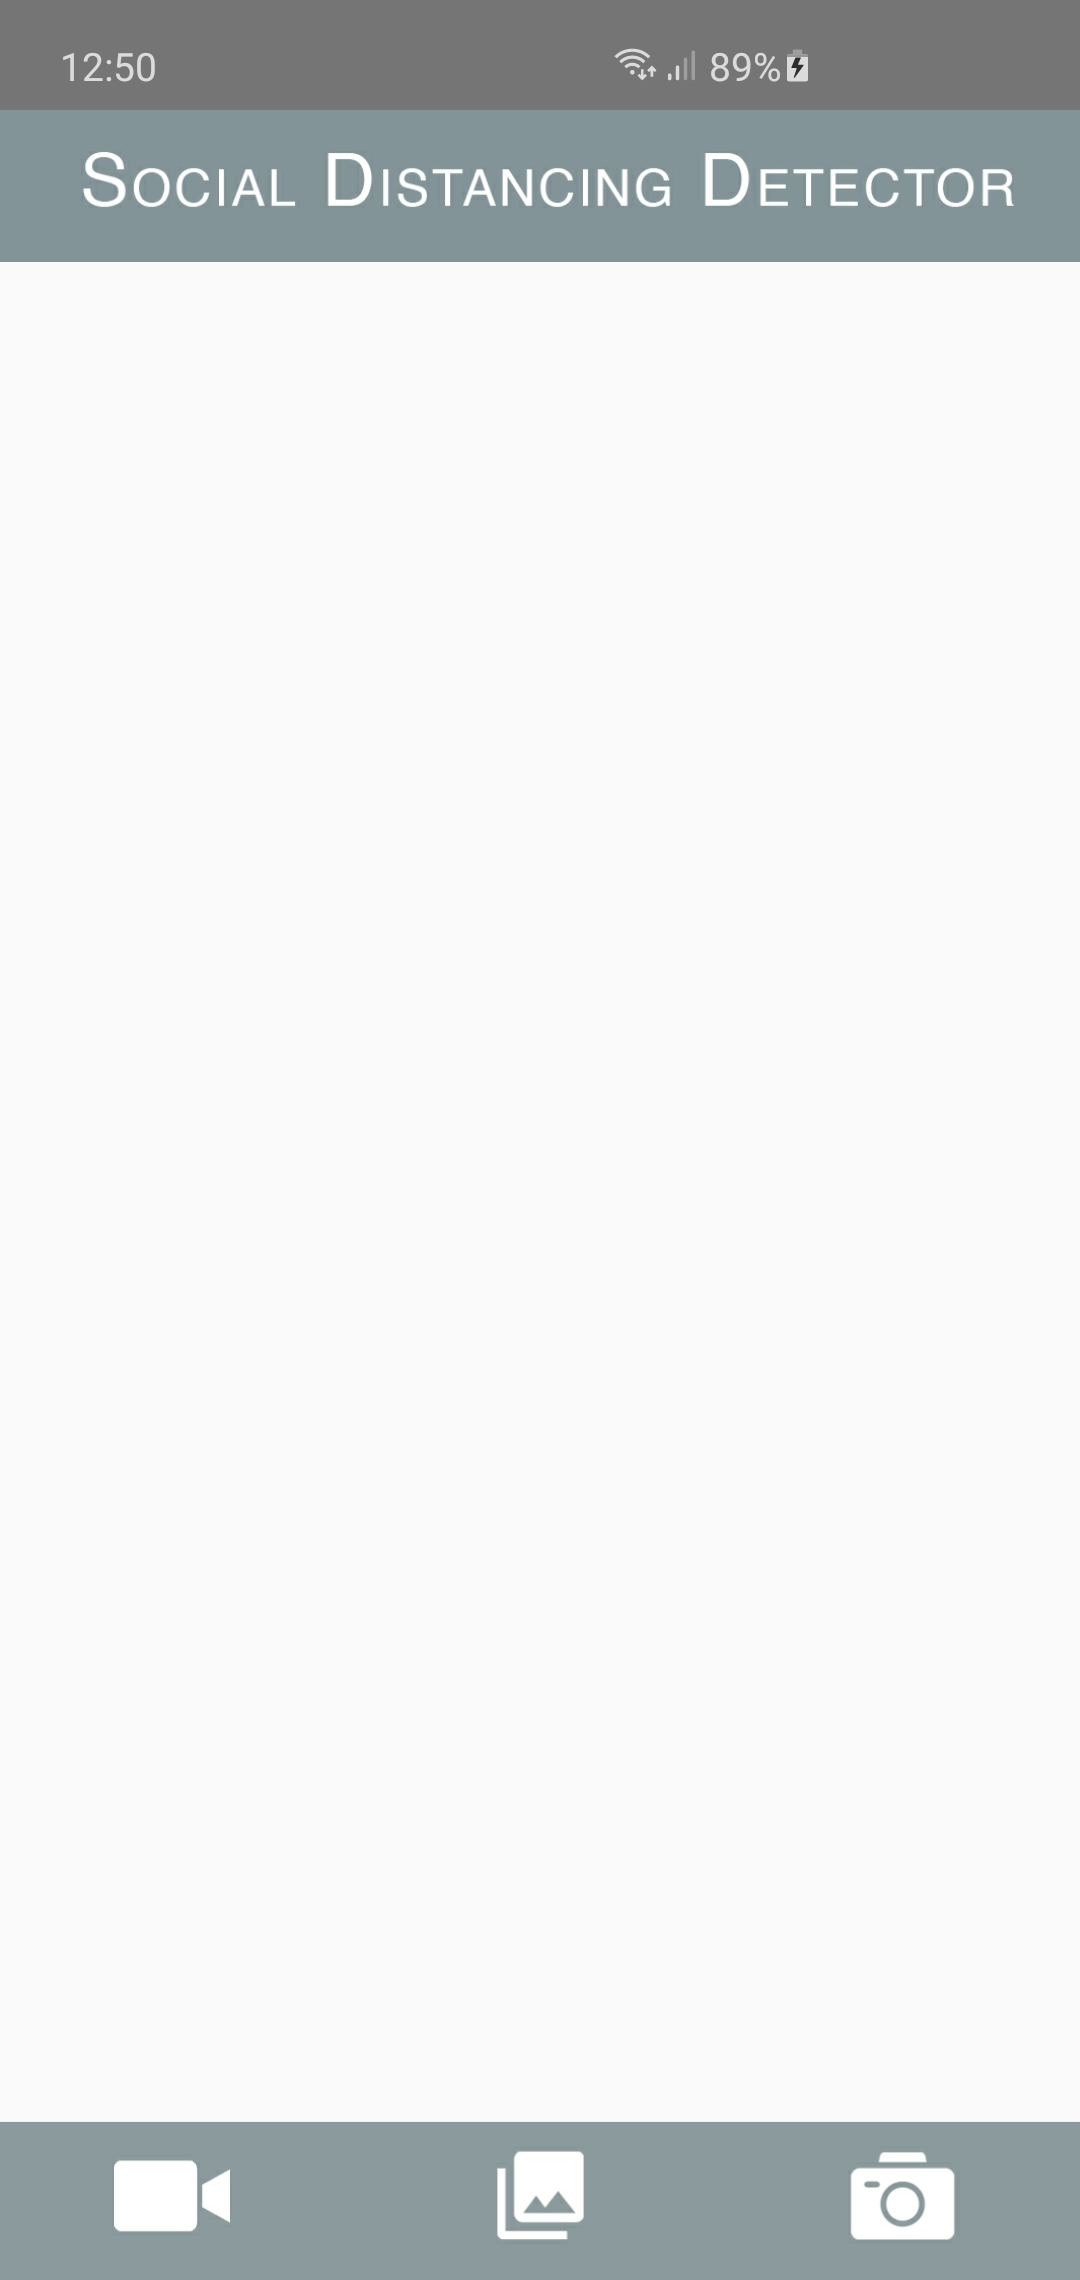
\includegraphics[width=1.5in]{images/appendix-b/sh-main.jpg}
        \caption{Main Menu}
        \label{appendix-b:mainMenu}
        \end{subfigure}%
        \begin{subfigure}{.5\textwidth}
        \centering
        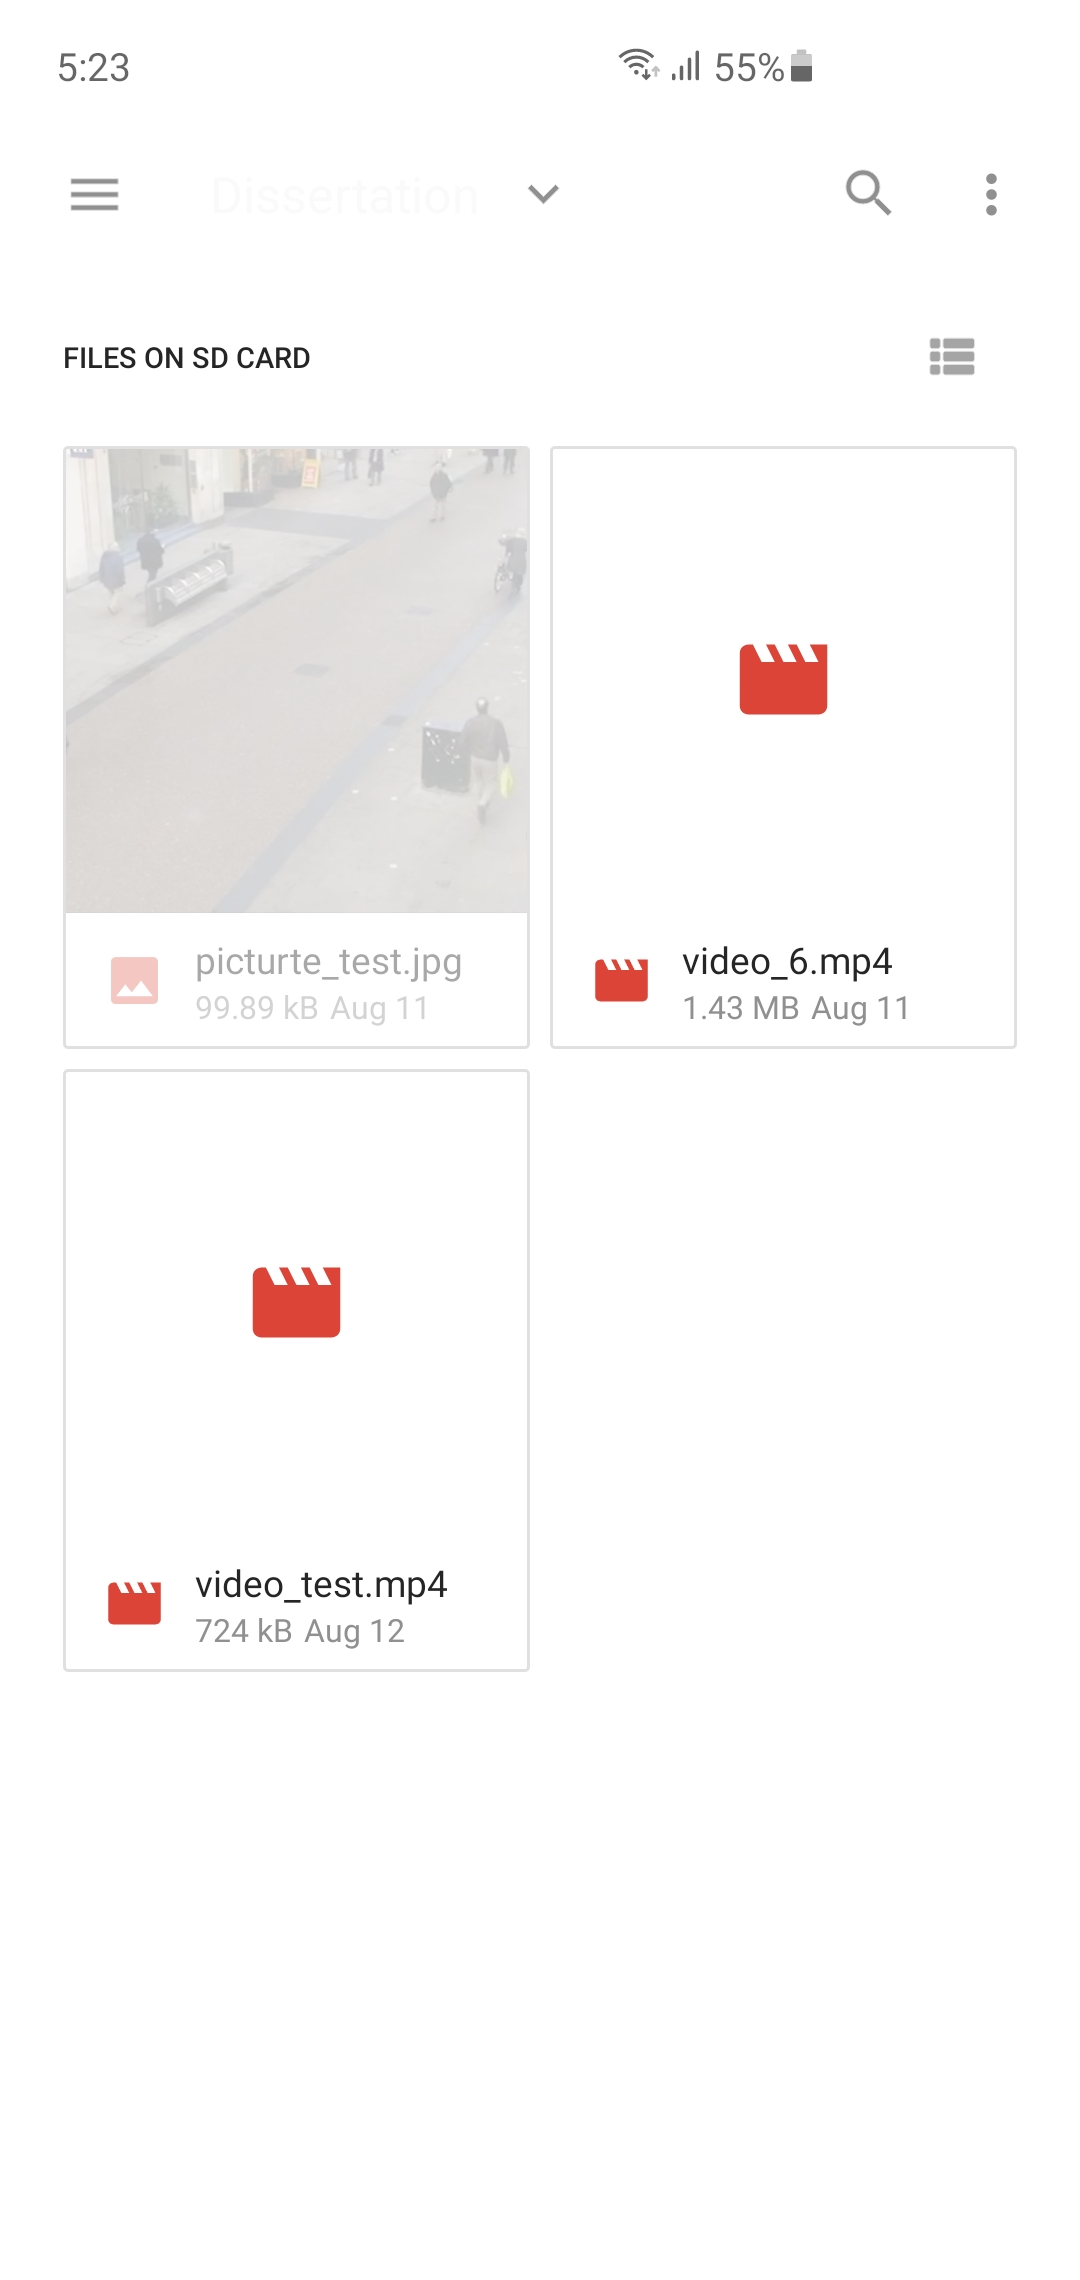
\includegraphics[width=1.5in]{images/appendix-b/sh-choosing.jpg}
        \caption{Choosing Existing File from Gallery}
        \label{appendix-b:filePicker}
        \end{subfigure}
        \caption{Application Interface}
        \label{appendix-b:menu}
    \end{figure}

    \begin{figure}[h!]
        \centering
        \begin{subfigure}{.5\textwidth}
        \centering
        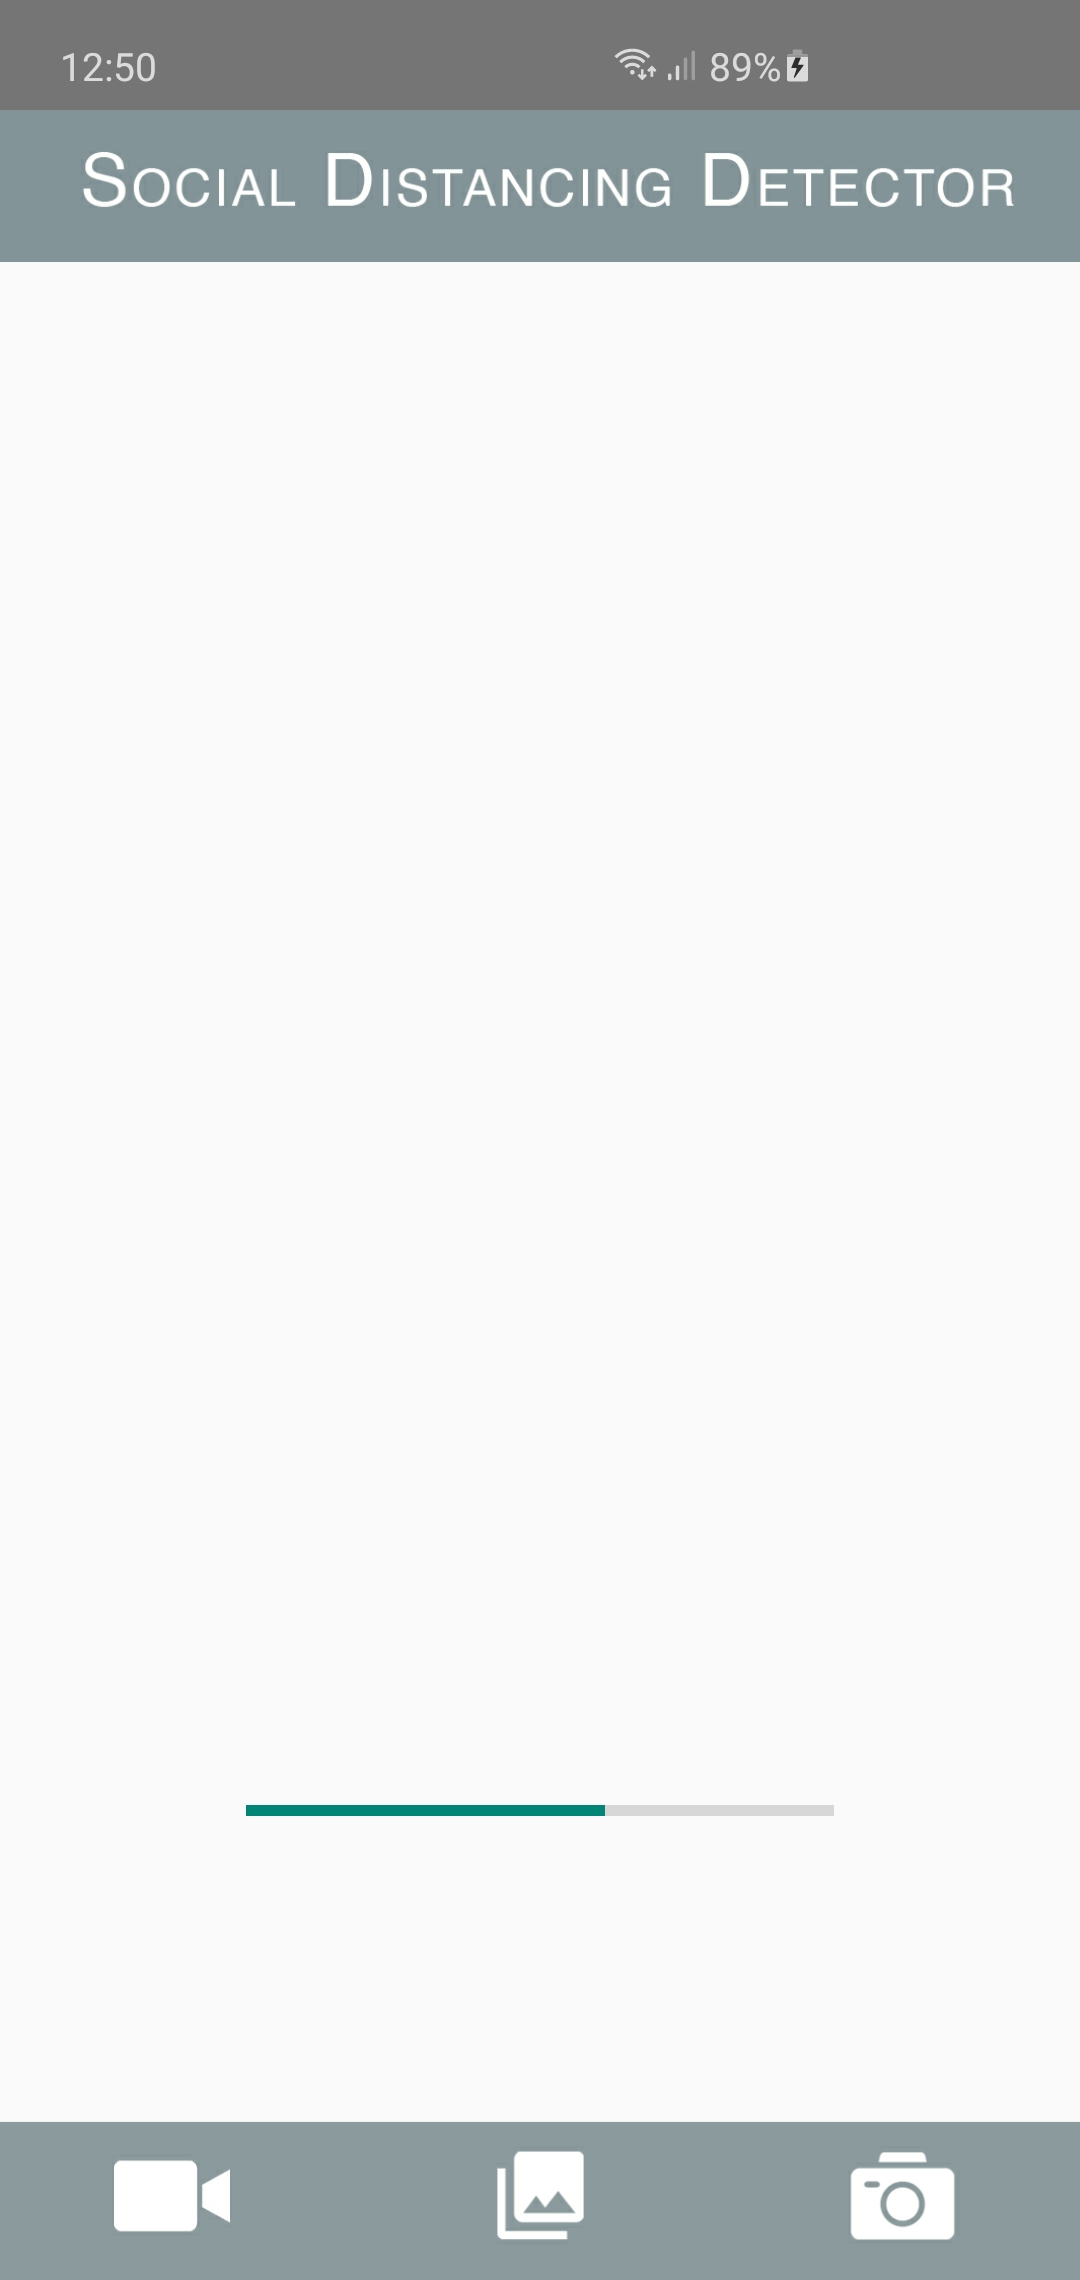
\includegraphics[width=1.5in]{images/appendix-b/sh-processing.jpg}
        \caption{Status Bar While Processing}
        \label{appendix-b:statusBar}
        \end{subfigure}%
        \begin{subfigure}{.5\textwidth}
        \centering
        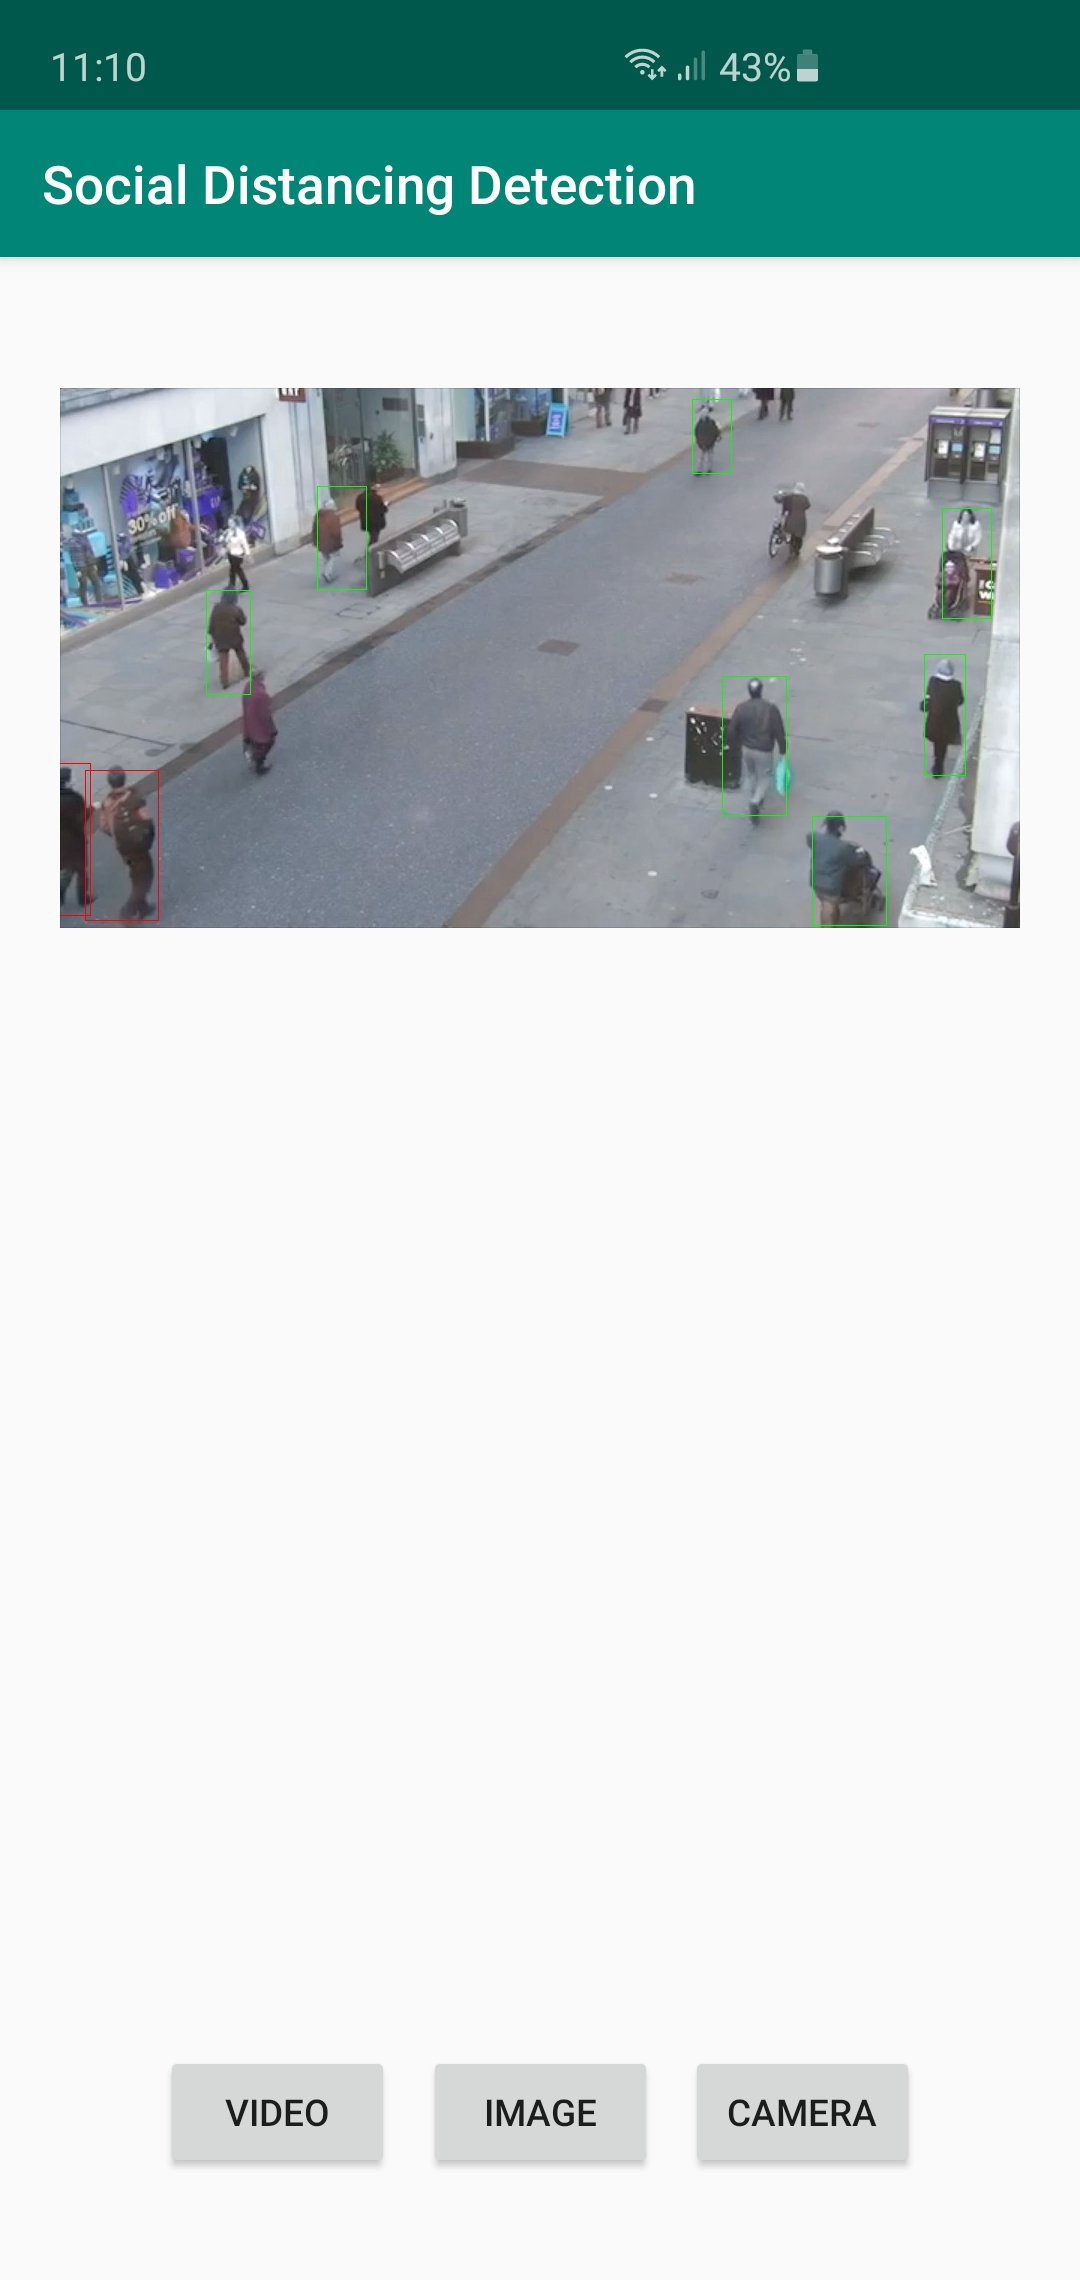
\includegraphics[width=1.5in]{images/appendix-b/sh-output.jpg}
        \caption{Display a proessed image or video}
        \label{appendix-b:result}
        \end{subfigure}
        \caption{Processing pre-recorded file}
        \label{appendix-b:process}
    \end{figure}

    \begin{figure}[!ht]
        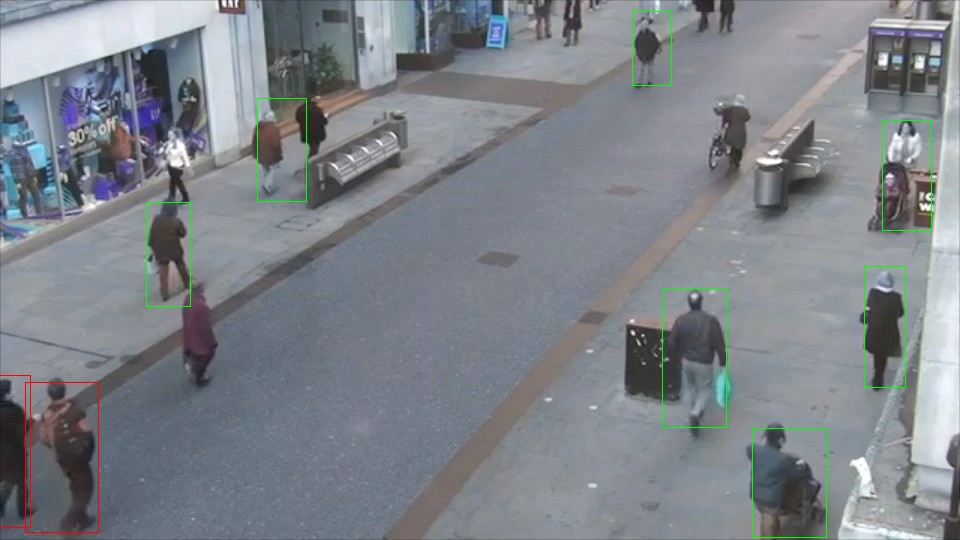
\includegraphics[width=6in]{images/chapter5/application/picture-detection.jpg}
        \caption{Social Distancing Detection from Picture}
        \label{appendix-b:sampleResult}
    \end{figure}

    \begin{figure}[!ht]
        \centering
        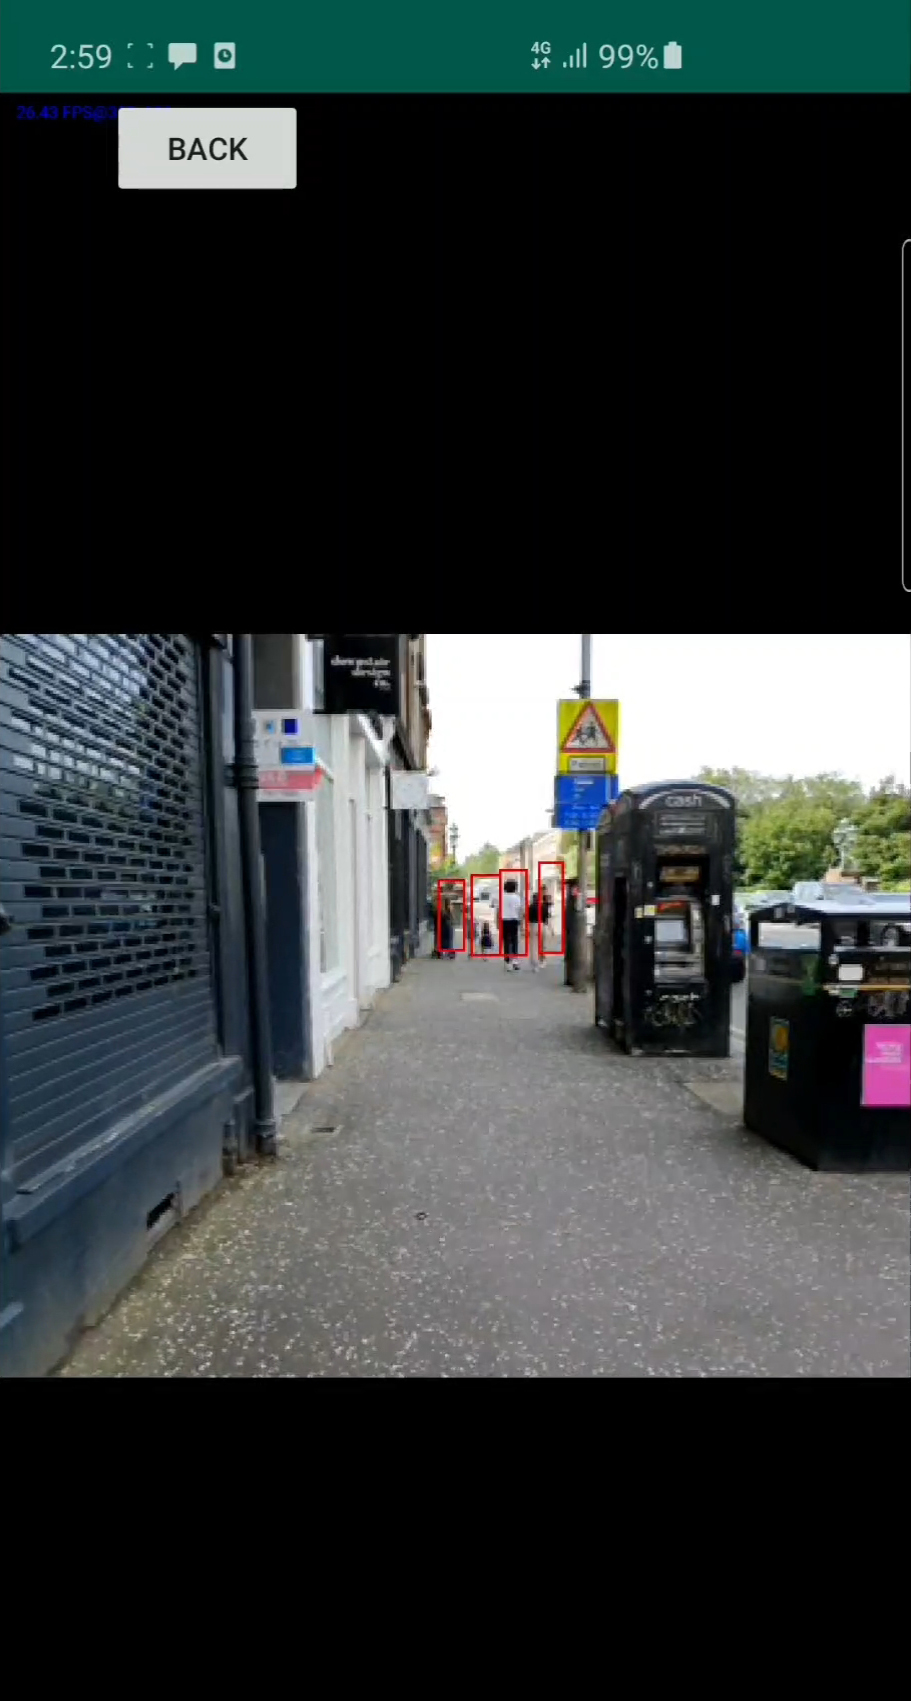
\includegraphics[width=2.5in]{images/chapter5/application/camera-detection.jpg}
        \caption{Social Distancing Detection by Using Camera}
        \label{appendix-b:camera}
    \end{figure}